% vim: set tw=80 aw sw=2 sts=2 noet:
\documentclass{beamer}

%\includeonlyframes{c} % speeding up compilation speed during debug

\usepackage[utf8x]{inputenc} % diacritice
\PrerenderUnicode{ĂăâÂîÎșȘțȚ}
\usepackage[romanian]{babel}
\usepackage{hyperref}        % \url{http://...} | \href{http://...}{Nume Link}

\usepackage{graphicx}% http://ctan.org/pkg/graphicx
\usepackage{booktabs}% http://ctan.org/pkg/booktabs
\pdfobjcompresslevel=0 
% Pentru a include cod decomentati urmatoarele 3 linii
%\usepackage{color}			 % highlight
%\usepackage{alltt}			 % highlight
%\usepackage{code/highlight}	 % highlight

\usepackage[absolute,overlay]{textpos}
  \setlength{\TPHorizModule}{1mm}
  \setlength{\TPVertModule}{1mm}


\mode<presentation>
\usetheme{SCS}

% Pentru a afisa (cont.) la slide-uri prea lungi split-uite pe mai multe pag
\setbeamertemplate{frametitle continuation}[from second]
% Pentru a modifica modul de afisare al numerelor de slide
\setbeamertemplate{footline}[frame number]

\title{Malsharp: Malicious Application Analysis}
\subtitle{Bachelor Thesis, July 2013}
% Folositi institutul pentru conducatorul stiintific
\institute{\small{As.dr.ing. Laura Gheorghe}}
\author{\small{Cristian Condurache}}

\begin{document}

{
  % Schimbam fundalul aici pentru a avea slide-ul cu logo-urile
  % Nu știu momentan cum se face asta în template.
  \usebackgroundtemplate{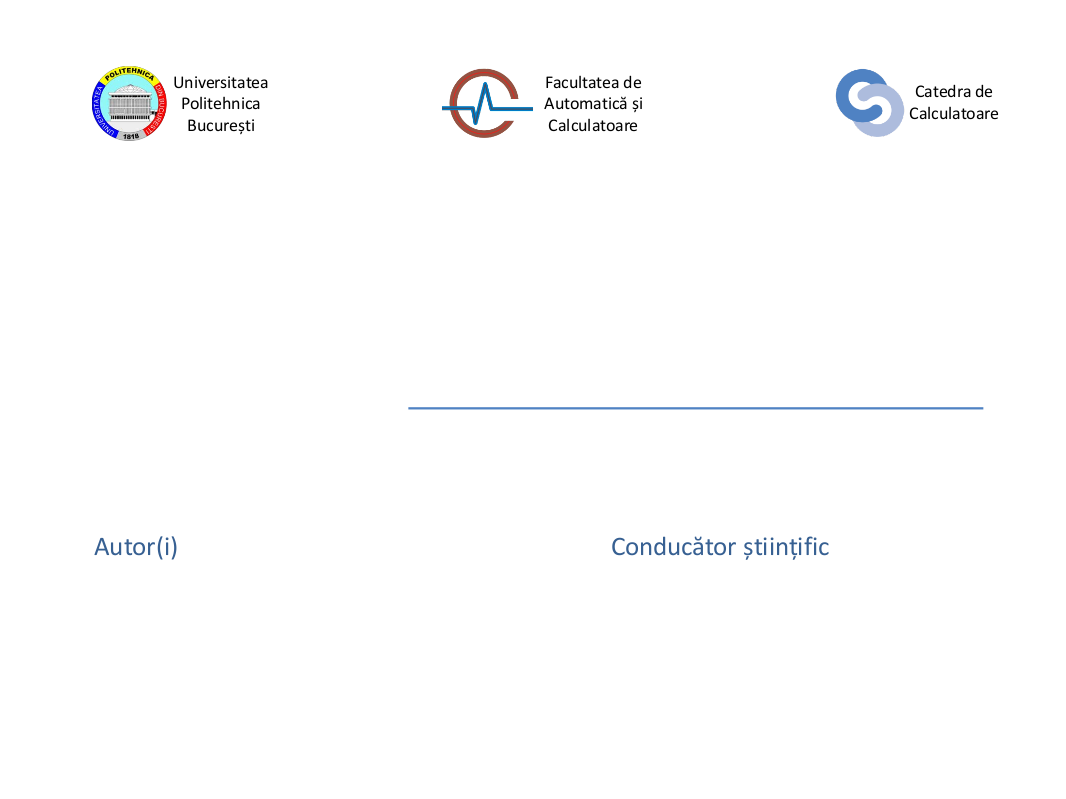
\includegraphics[width=\paperwidth]{title}}
  \frame{\titlepage}
}

\begin{frame}{Motivation \& Goals}
  \begin{itemize}
    \item<1-> Why?
    \begin{itemize}
      \item[--] Popularity of Linux based OSs
      \item[--] Use in embedded systems
    \end{itemize}
    \item<2-> How?
    \begin{itemize}
      \item[--] Malsharp: malicious behavior pattern mining
    \end{itemize}
  \end{itemize}
\end{frame}

\begin{frame}{Malware Detection}
  \begin{itemize}
    \item Signature-based
    \begin{itemize}
      \item[--] Problem: fails to detect new malware, obfuscation
    \end{itemize}
    \item Behavior-based
    \begin{itemize}
      \item[--] Problem: behavior patterns require manual identification
    \end{itemize}
  \end{itemize}
\end{frame}

\begin{frame}{Malspec Mining Algorithm}
  \begin{itemize}
    \item<1-> Input: a malware sample and a set of benign programs
    \item<2-> Output: a malicious behavior pattern
    \item<3-> Creates graphs for sample malware and benign programs
    \begin{itemize}
      \item[--] A node represents a system call
      \item[--] An edge is an argument dependency
    \end{itemize}
    \item<4-> Computes malware specifications as ``difference'' between graphs
    \begin{itemize}
      \item[--] Maximal common subgraph algorithm
      \item[--] Complement graph
      \item[--] Minimal transversal
    \end{itemize}
  \end{itemize}
\end{frame}

\begin{frame}{Dependency Graph (1)}
  \begin{itemize}
    \item Initial nodes
  \end{itemize}
  \begin{figure}[p]
    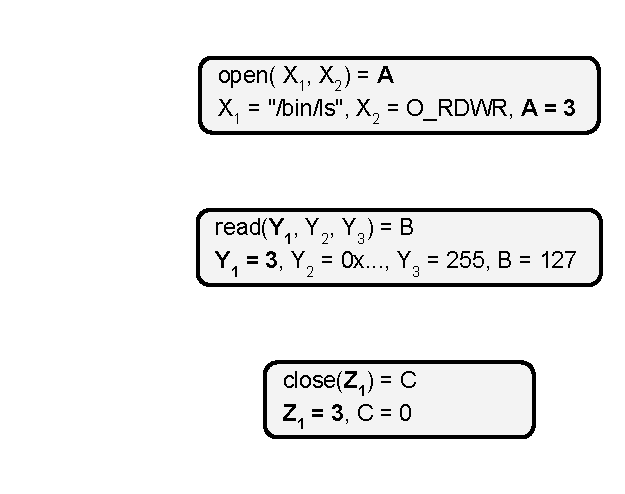
\includegraphics[width=3in]{img/syscall-dep-graph-0.pdf}
    \end{figure}
\end{frame}

\begin{frame}{Dependency Graph (2)}
  \begin{itemize}
    \item Adding a dependency edge between open and read
  \end{itemize}
  \begin{figure}[p]
    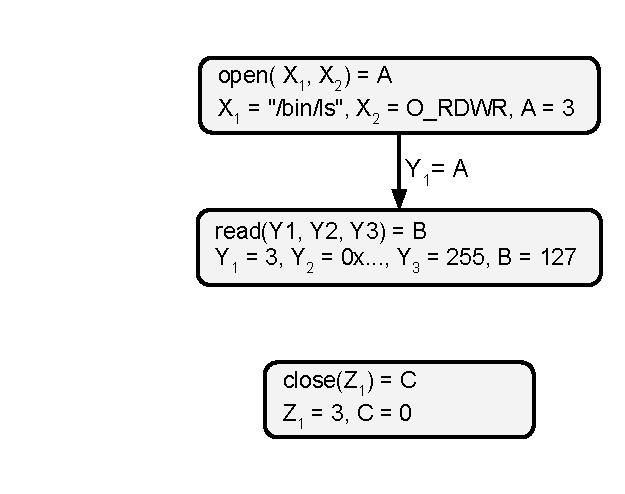
\includegraphics[width=3in]{img/syscall-dep-graph-1.pdf}
%    \caption{}
    \end{figure}
\end{frame}

\begin{frame}{Dependency Graph (3)}
  \begin{itemize}
    \item Adding a dependency edge between open and close
  \end{itemize}
  \begin{figure}[p]
    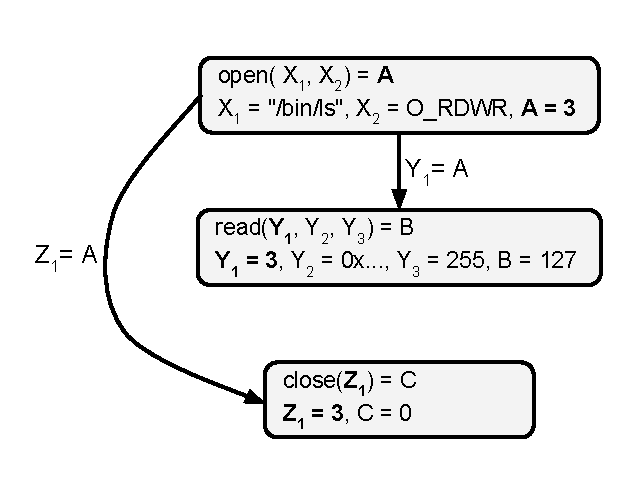
\includegraphics[width=3in]{img/syscall-dep-graph-2.pdf}
%    \caption{}
    \end{figure}
\end{frame}

\begin{frame}[t]{Malsharp Architecture}
  \begin{figure}[p]
    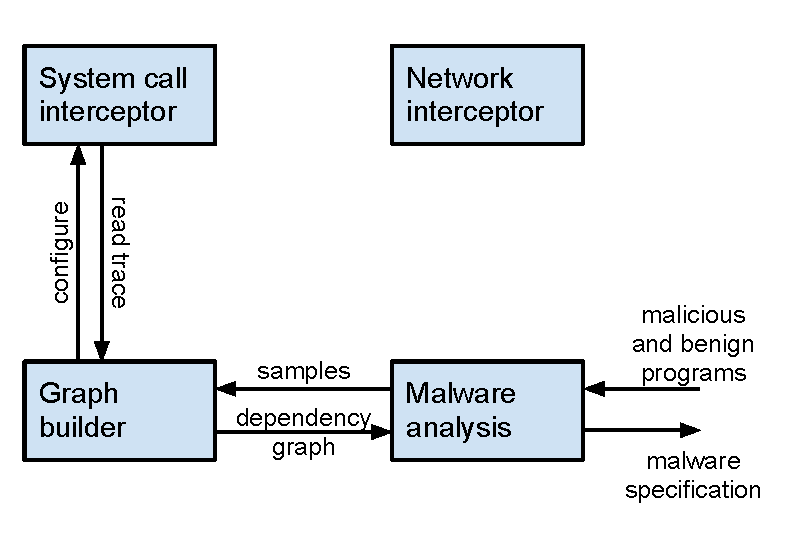
\includegraphics[width=4.4in]{img/mal-sharp-architecture.pdf}
    \end{figure}
\end{frame}

\begin{frame}[t]{Implementation (1)}
  \begin{figure}[ht]
    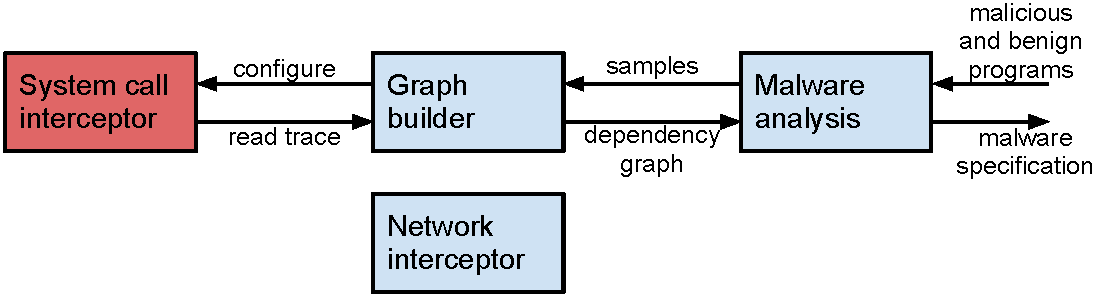
\includegraphics[width=4.4in]{img/mal-sharp-architecture-scid.pdf}
    \end{figure}
  \begin{itemize}
    \item System Call Interceptor Driver (SCID)
    \begin{itemize}
      \item[--] Logs execution trace for a process
      \item[--] Kernel module, registers by using miscdevice
      \item[--] Controlled via the ioctl system call
    \end{itemize}
  \end{itemize}
\end{frame}

\begin{frame}[t]{Implementation (2)}
  \begin{figure}[p]
    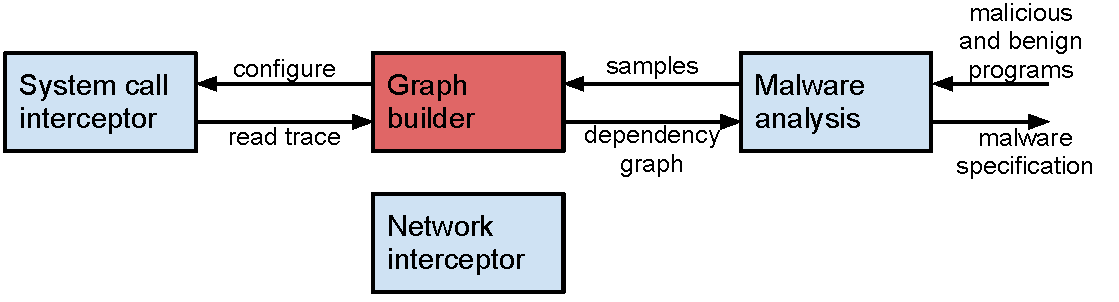
\includegraphics[width=4.4in]{img/mal-sharp-architecture-gb.pdf}
  \end{figure}
  \begin{itemize} 
    \item Graph Builder
    \begin{itemize}
      \item[--] Runs each program
      \item[--] Reads execution traces from SCID
      \item[--] Finds argument dependencies
      \item[--] Node aggregation: a read of 1000 bytes is equivalent to 1000 individual reads of 1 byte
    \end{itemize}
  \end{itemize}
\end{frame}

\begin{frame}[t]{Implementation (3)}
  \begin{figure}[p]
    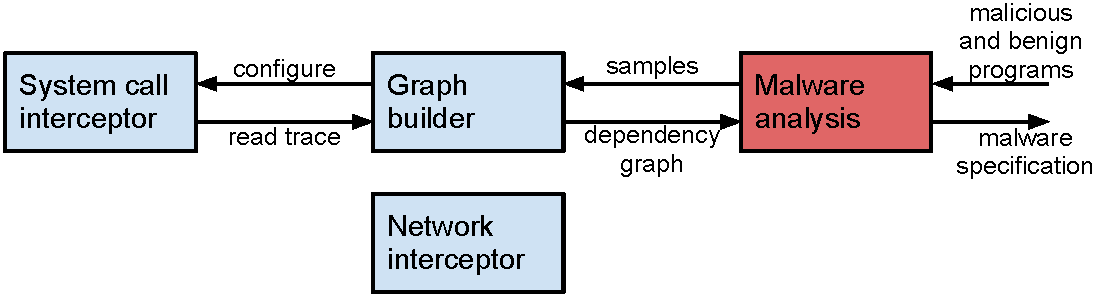
\includegraphics[width=4.4in]{img/mal-sharp-architecture-ma.pdf}
  \end{figure}
  \begin{itemize}
    \item Malware Analysis
    \begin{itemize}
      \item[--] Uses the graph builder for each program
      \item[--] Applies the malspec mining algorithm
    \end{itemize}
  \end{itemize}
\end{frame}

\begin{frame}[t]{Implementation (4)}
  \begin{figure}[p]
    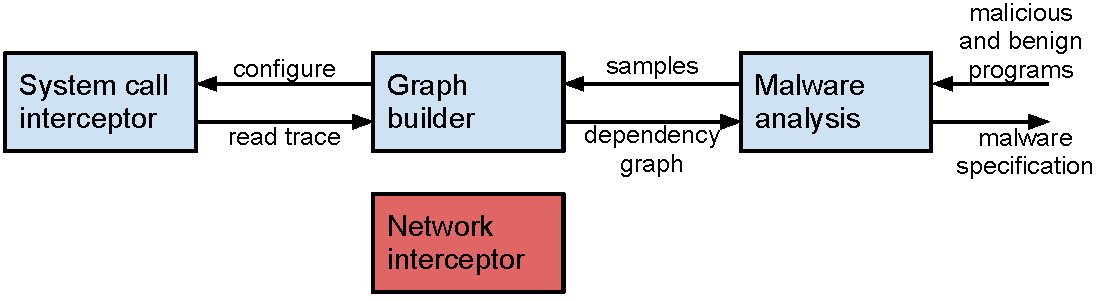
\includegraphics[width=4.4in]{img/mal-sharp-architecture-ni.pdf}
    \end{figure}
  \begin{itemize}
    \item Network Interceptor (NI)
    \begin{itemize}
      \item[--] Used for monitoring malware networking activity
      \item[--] Netfilter hooks to monitor traffic
      \item[--] Can be configured to monitor specific protocols
    \end{itemize}
  \end{itemize}
\end{frame}

\begin{frame}{Evaluation (1)}
  \begin{itemize}
    \item<1-> Virtual machine, snapshots
    \item<1-> Bridged network access
    \item<1-> Revert to snapshot before each test
    \vspace{0.3cm}
    \item<2-> Monitored two sets of system calls
    \vspace{0.3cm}
    \item<3-> A set of 20 well-known malware samples
    \begin{itemize}
      \item[--] Viruses: Virus.Linux.Rike.1627, Virus.Linux.Osf.8759
      \item[--] Backdoors: Backdoor.Linux.CGI, Backdoor.Linux.Phobi.1
    \end{itemize}
  \end{itemize}
\end{frame}

\begin{frame}{Evaluation (2)}
  \begin{itemize}
    \item Execution traces, graphs successfully built
    \item Malware patterns identified, 3-5 nodes
    \item Results for Virus.Linux.Radix
  \end{itemize}
  \begin{figure}[p]
    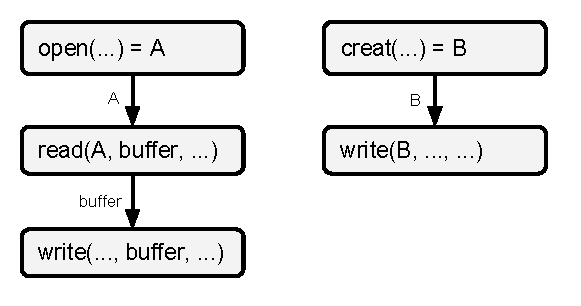
\includegraphics[width=3in]{img/malspec-result.pdf}
  \end{figure}
\end{frame}


\begin{frame}
  \frametitle{Evaluation (3)}
  \begin{center}
  \scriptsize{
  \begin{tabular}{lcccccc}
    \toprule
    Sample & Nodes & Edges & Malspec & Time & Observed behavior \\
    \midrule
    Backdoor.Linux.CGI.a   & 13  & 5   & 1 & 0.827s  & open, read, close  \\
    Backdoor.Linux.Phobi.1 & 35  & 16  & 1 & 0.641s  & open, read, close  \\
    Trojan.Linux.Rootkit.n & 14  & 5   & 1 & 1.044s  & open, read, close  \\
    Virus.Linux.Radix      & 22  & 6   & 1 & 0.673s  & open, read, write; \\ 
                           &     &     &   &         & creat, write       \\
    Virus.Linux.Svat.b     & 25  & 12  & 0 & 3.495s  & replaces stdio.h   \\
    \bottomrule
  \end{tabular}
  }
  \end{center}
\end{frame}

\begin{frame}{Node aggregation results}
  \begin{figure}[p]
    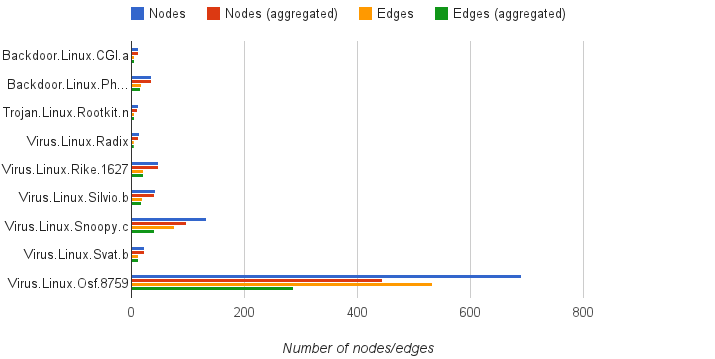
\includegraphics[width=5in]{img/node-aggregation-android.png}
  \end{figure}
\end{frame}

\begin{frame}{Memory usage}
  \begin{figure}[p]
    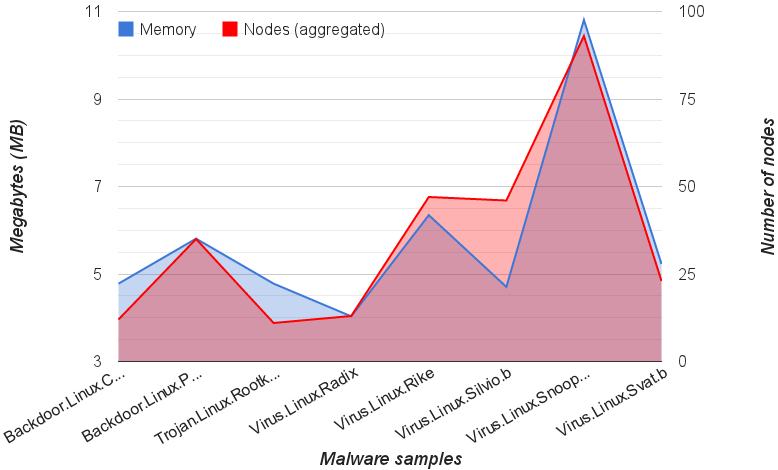
\includegraphics[width=4in]{img/mal-memory-use.png}
  \end{figure}
\end{frame}

\begin{frame}{Conclusions}
  \begin{itemize}
    \item Proof of concept for a Linux malware behavior miner
    \item Analysis detected malicious patterns
    \item Node aggregation successfully reduced total number of nodes
    \item Possible future improvements:
    \begin{itemize}
      \item[--] Additional pruning: node ordering strategies
      \item[--] Adding other types of dependency edges
    \end{itemize}
  \end{itemize}
\end{frame}

% ------------------------------------------------
%                    BONUS
% ------------------------------------------------

\begin{frame}{Test programs}
  \begin{figure}[p]
    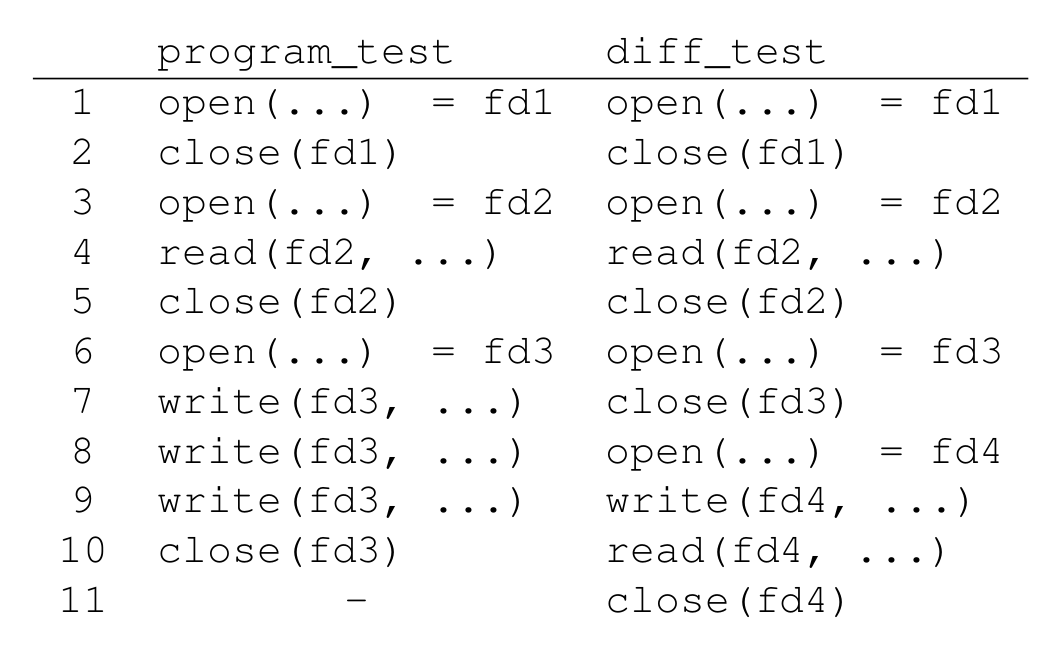
\includegraphics[width=3.6in]{img/programs.png}
%    \caption{}
    \end{figure}
\end{frame}

\begin{frame}{Maximal common edge set}
  \begin{figure}[p]
    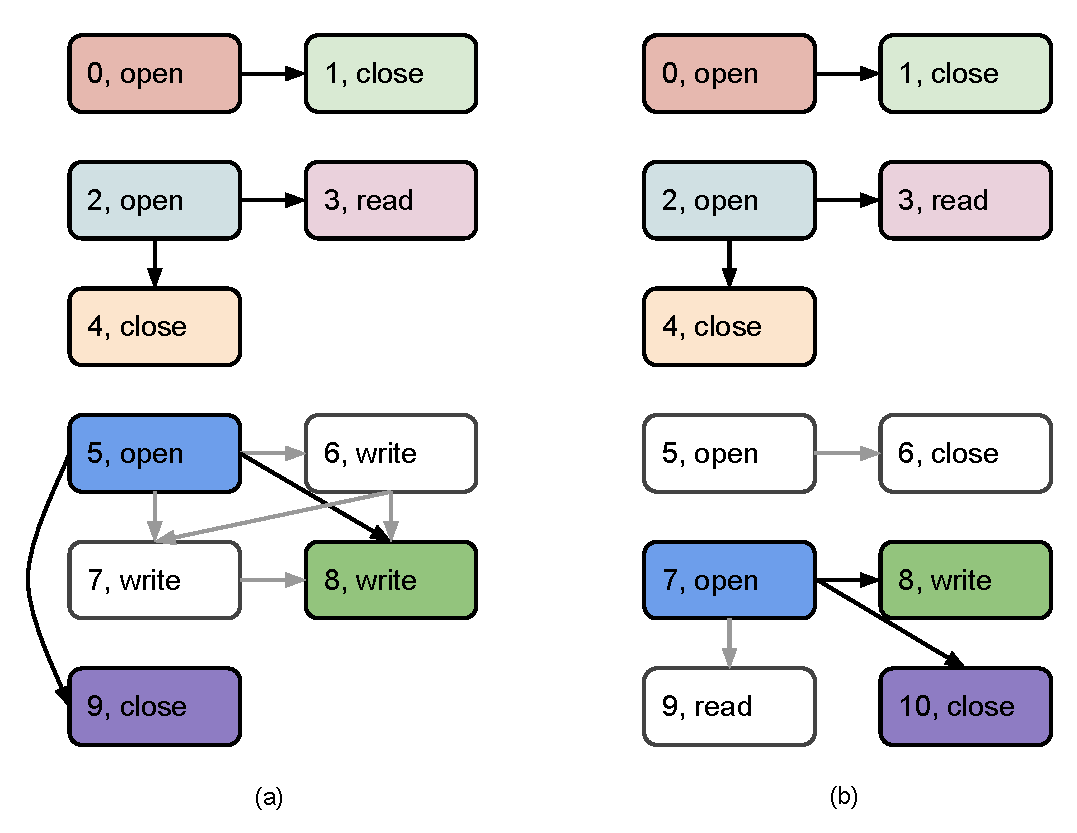
\includegraphics[width=3.6in]{img/max-common-edge-set.pdf}
%    \caption{}
    \end{figure}
\end{frame}

\begin{frame}{Complement and minimal transversal}
  \begin{figure}[p]
    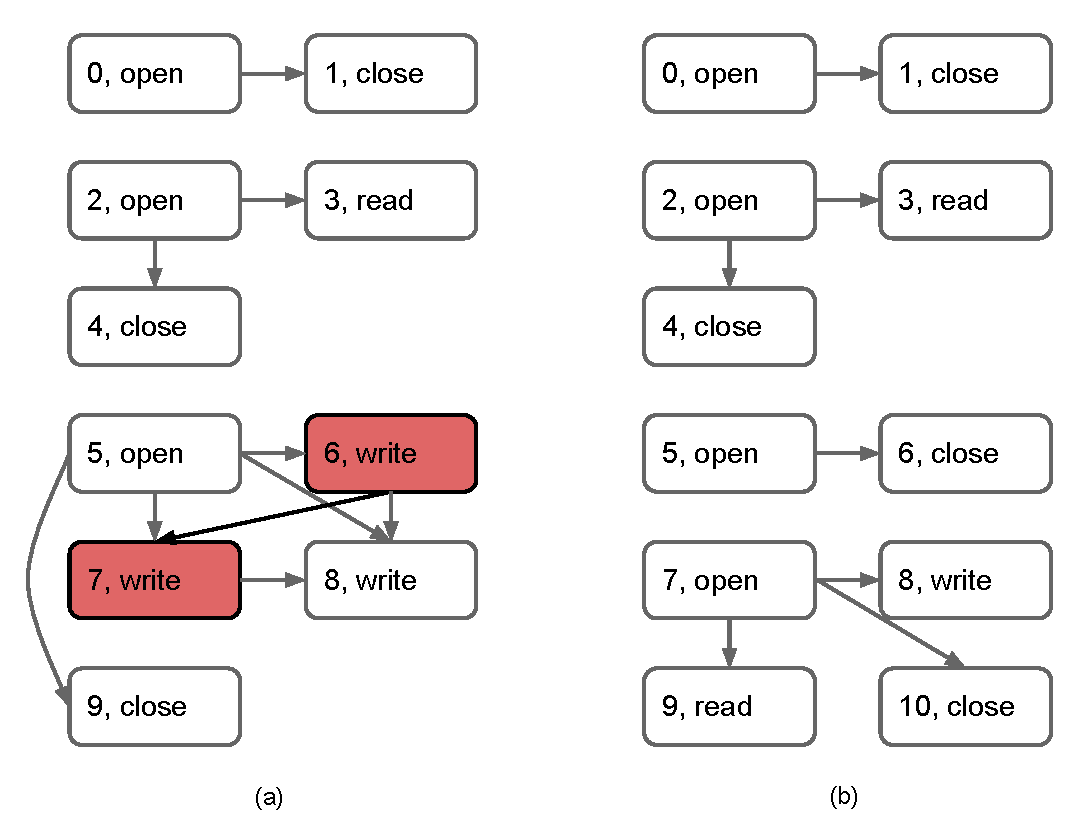
\includegraphics[width=3.6in]{img/min-transversal-compl.pdf}
%    \caption{}
    \end{figure}
\end{frame}

\end{document}

